%\documentclass[11pt,a4paper,uplatex,twoside,dvipdfmx]{ujarticle} 	% for uplatex
\documentclass[11pt,a4paper,twoside,dvipdfmx]{jarticle}		% platex
%==== 科研費LaTeX =============================================
%	2021(R03)年度 海外特別研究員
%============================================================
% 2009-03-07: Taku Yamanaka (Osaka Univ.)
%			Copied over from PD.
% 2011-03-20: Taku Yamanaka
%			Made a 2012 version.
% 2012-02-25: Taku: Made 2013 version.
% 2013-03-15: Taku: Made 2014 version.
% 2014-03-02: Taku: Made 2015 version.
% 2015-02-22: Taku: Made 2016 version.
% 2016-03-16: Taku: Made 2017 version.
%============================================================
%=======================================
% form00_header.tex
%	General header for kakenhiLaTeX,  Moved over from form00_2010_header.tex.
%	2009-09-06 Taku Yamanaka (Osaka Univ.)
%==== General Version History ======================================
% 2006-05-30 Taku Yamanaka (Physics Dept., Osaka Univ.)
% 2006-06-02 V1.0
% 2006-06-14 V1.1 Use automatic calculation for cost tables.
% 2006-06-18 V1.2 Split user's contents and the format.
% 2006-06-20 V1.3 Reorganized user and format files
% 2006-06-25 V1.4 Readjusted all the table column widths with p{...}.
%				With \KLTabR and \KLTabRNum, now the items can be right-justified
%				in the cell defined by p{...}.
% 2006-06-26 V1.5 Use \newlength and \setlength, instead of \newcommand, to define positions.
% 2006-08-19 V1.6 Remade it for 2007 JFY version.
% 2006-09-05 V1.7 Added font declarations suggested by Hoshino@Meisei Univ.
% 2006-09-06 V1.8 Introduced usePDFform flag to switch the form file format.
% 2006-09-09 V1.9 Changed p.7, to allow different heights between years. (Thanks to Ytow.)
% 2006-09-11 V2.0 Added an option to show budget summary.
% 2006-09-13 V2.1 Added an option to show the group.
% 2006-09-14 V2.1.1 Cleaned up Kenkyush Chosho.
% 2006-09-21 V2.2 Generated under a new automatic development system.

% 2007-03-24 V3.0 Switched to a method using "picture" environment.

% 2007-08-14 V3.1 Switched to kakenhi3.sty.
% 2007-09-17 V3.2 Added \KLMaxYearCount
% 2008-03-08 V3.3 Remade it for 2009 JFY version\
% 2008-09-08 V3.4 Added \KLXf ... \KLXh.
% 2011-10-20 V5.0 Use kakenhi5.sty, to utilize array package in tabular environment.
% 2012-08-14 v5.1 Moved preamble and kakenhi5 into the current directory, instead of the parent directory.
% 2012-11-10 v6.0 Switched to kakenhi6.sty.
% 2015-08-26 v6.1 Added KLFirstPageIsLongPage flag.
% 2018-02-12 Taku: Commented out \DeclareFontShape ...
%=======================================
%============================================================
% preamble.tex
%
% Dummy section and subsection commands.
% With these, some editors (such as TeXShop, etc.) can jump to the (sub)sections.
\newcommand{\dummy}{dummy}% 
\renewcommand{\section}[1]{\renewcommand{\dummy}{#1}}
\renewcommand{\subsection}[1]{\renewcommand{\dummy}{#1}}

% Flag for switching form file format.......
\usepackage{ifthen}
\newboolean{usePDFform}
\newboolean{BudgetSummary}

\usepackage{forms/kakenhi6}

\pagestyle{empty}

% ===== Parameters for LaTeX =========================

% ===== Font declarations  ======================================
%%\DeclareFontShape{JT1}{mc}{m}{it}{<->ssub * mc/m/n}{}
%%\DeclareFontShape{JY1}{mc}{m}{it}{<->ssub * mc/m/n}{}

% ===== Parameters for KL (Kakenhi LaTeX) ========================
% general purpose temporary variables	-2007
\newcommand{\KLX}{}
\newcommand{\KLXa}{}
\newcommand{\KLXb}{}
\newcommand{\KLXc}{}
\newcommand{\KLXd}{}
\newcommand{\KLXe}{}
\newcommand{\KLXf}{}
\newcommand{\KLXg}{}
\newcommand{\KLXh}{}
\newcommand{\KLY}{}
\newcommand{\KLYa}{}
\newcommand{\KLYb}{}
\newcommand{\KLYc}{}
\newcommand{\KLYd}{}
\newcommand{\KLYe}{}
\newcommand{\KLYf}{}
\newcommand{\KLXR}{}
\newlength{\KLCella}
\newlength{\KLCellb}
\newlength{\KLCellc}
\newlength{\KLCelld}
\newlength{\KLCelle}
\newlength{\KLCellf}
\newlength{\KLCellg}
\newlength{\KLCellh}

% sub-page
\newlength{\KLSubPageX}
\newlength{\KLSubPageY}
\newlength{\KLspx}
\newlength{\KLspy}
\newcommand{\KLSubPageXmm}{}	% for \input(x,y){....} which uses a unit (mm)
\newcommand{\KLSubPageYmm}{}	% for \input(x,y){....} which uses a unit (mm)

% margins for parbox inside frames; in units of points
\newcounter{KLParboxSideMargin}
\newcounter{KLParboxTopMargin}
\newcounter{KLParboxBottomMargin}

% ===== standard counters ======================================
\newcounter{KLSubPageNo}	% sub-page counter
\newcounter{KLPageOffset}		% to generate sub-page number
\newcounter{KLMaxYearCount}	% # of years for the proposal

% ===== standard flags ============================
\newboolean{KLFirstPageIsLongPage}

% ===== initializations ============
\KLInitTypesettingPageSelection
\newcommand{\KLCLLang}{}	% language-dependent left-justification in tabular



% user01_header
%=== 様式のファイルの形式の指定 =================
%   PDFではなく、eps の様式を読み込む場合は、次の行の頭に「%」をつけてください。
\setboolean{usePDFform}{true}
%===================================
%==========================================================
% form01_header.tex
%	2014-03-02: Taku Yamanaka (Osaka Univ.)
%		This is called after usePDFform is set.
%		Originally, this part was in form07_header.tex, but then
%		\usepackage{color} that is called before it was not effective.
%		[dvipdfmx] is not used for eps forms, because it makes the forms
%		slightly larger than pdf forms.
%		
%==========================================================
% ===== File format for forms ===========================
\ifthenelse{\boolean{usePDFform}}{
	\newcommand{\KLFormFormat}{pdf}	\usepackage[dvipdfmx]{graphicx}
}{	\newcommand{\KLFormFormat}{eps}	\usepackage{graphicx}
}

%----------------------------------------------------------------------------


% user02_header
%=== 予算の表の印刷 =====================
% 予算の集計の表を出すためには、次の行の頭の%を消してください。
%\setboolean{BudgetSummary}{true}
%=================================

%=== For English, uncomment the next line to left-justify inside table columns.
%\renewcommand{\KLCLLang}{\KLCL}

% === 一部のページだけタイプセット ==============
% New in 2009 fall version!
% 選んだページだけタイプセットするには、次の例の頭の%を消し、並べてください。
% 複数のページを選ぶこともできます。
% 提出前には、必ず全てコメントアウト(頭に%をつける)してください。
%ーーーーーーーーーーーーーーーーーーーーーーーーーーーーーーーーー
%\KLTypesetPage{1}			% p.1 (or p.1を含む連続したページ),
%\KLTypesetPage{3}			% p.3 (or p.3を含む連続したページ),
%\KLTypesetPagesInRange{5}{6}	% p.5 ~ p.6,
%\KLTypesetPagesInRange{8}{10}	% and p.8 ~ p.10
%=================================

% ===== my favorite packages ====================================
% ここに、自分の使いたいパッケージを宣言して下さい。
\usepackage{wrapfig}
% \usepackage{amssymb}
%\usepackage{mb}
% \usepackage{color} % でも科研費の書類はグレースケールで印刷されます
%\DeclareGraphicsRule{.tif}{png}{.png}{`convert #1 `dirname #1`/`basename #1 .tif`.png}
%==========================================================

\newcommand{\KLShouKeiLine}[1]{\cline{#1}}
%もし、小計の上の線を取れと事務に言われたら、
%「そのようなことは、記入要項に書かれていないし、学振はそのようなことは気にしていない。」と
% 突っぱねる。
% それでもなお消せと理不尽なことを言われたら、次の行の 最初の「%」を消す。	
%\renewcommand{\KLShouKeiLine}[1]{}

\newcommand{\KLBudgetTableFontSize}{small}	% 予算の表のフォントの大きさ: small, footnotesize
\newcommand{\KLFundsTableFontSize}{small}	%応募中、受入れ予定の研究費のフォントの大きさ:normalsize, small, footnotesize

% ===== my personal definitions ==================================
% ここに、自分のよく使う記号などを定義して下さい。
\newcommand{\klpionn}{K_L \to \pi^0 \nu \overline{\nu}}
\newcommand{\kppipnn}{K^+ \to \pi^+ \nu \overline{\nu}}


% hook3: after including packages ===================
 % for future maintenance
% ===== Global definitions for the PD form ======================
% 基本情報
%
%------ 研究課題名  -------------------------------------------
\newcommand{\研究課題名}{象の卵}

%----- 研究機関名と研究代表者の氏名-----------------------
\newcommand{\研究機関名}{逢坂大学}
\newcommand{\申請者氏名}{湯川秀樹}
\newcommand{\研究代表者氏名}{\申請者氏名}

%---- 研究期間の最終年度 ----------------
\newcommand{\研究期間の最終元号年度}{34}	%平成で、半角数字のみ
%=========================================================
% ===== Global year-dependent definitions for the Kakenhi form ===========
% 基本情報
\newcommand{\研究開始年度}{2021}
\newcommand{\研究開始元号年度}{03}	%令和

\newcommand{\一年目西暦}{2021}
\newcommand{\二年目西暦}{2022}
\newcommand{\三年目西暦}{2023}
\newcommand{\四年目西暦}{2024}
\newcommand{\五年目西暦}{2025}
\newcommand{\六年目西暦}{2026}

\newcommand{\一年目}{3}
\newcommand{\二年目}{4}
\newcommand{\三年目}{5}
\newcommand{\四年目}{6}
\newcommand{\五年目}{7}
\newcommand{\六年目}{8}

\newcommand{\一年目J}{3}
\newcommand{\二年目J}{4}
\newcommand{\三年目J}{5}
\newcommand{\四年目J}{6}
\newcommand{\五年目J}{7}
\newcommand{\六年目J}{8}


	% <<<
%==========================================================
% form03_header.tex
%	2009-03-04: Taku Yamanaka (Osaka Univ.)
%==========================================================
\usepackage{calc}
\usepackage{watermark}
\usepackage{longtable}
\usepackage{geometry}                % See geometry.pdf to learn the layout options. There are lots.
\usepackage{udline}
\usepackage{array}

\geometry{noheadfoot,scale=1}  %scale=1 resets margins to 0
\setlength{\unitlength}{1pt}

% define variables for positions ==========================
% picture environment location, in  units of points
\newcommand{\KLOddPictureX}{}
\newcommand{\KLEvenPictureX}{}
\newcommand{\KLPictureY}{}
\newcommand{\KLOddPictureInWaterMarkX}{}
\newcommand{\KLEvenPictureInWaterMarkX}{}
\newcommand{\KLPictureInWaterMarkY}{}

\newlength{\KLoddsidemargin}
\newlength{\KLevensidemargin}
\newlength{\KLtopmargin}

\newcounter{KLCOddPictureInWaterMarkX}
\newcounter{KLCEvenPictureInWaterMarkX}
\newcounter{KLCPictureInWaterMarkY}
\newcounter{KLCOddPictureX}
\newcounter{KLCEvenPictureX}
\newcounter{KLCPictureY}

%------------------------------------------------------------

\newcommand{\KLLeftEdge}{}
\newcommand{\KLRightEdge}{}

% standard margins for text in frames
\setcounter{KLParboxSideMargin}{7}
\setcounter{KLParboxTopMargin}{12}
\setcounter{KLParboxBottomMargin}{5}

%-----------------------------------------------------------
\newcommand{\KLTwoHLines}{\hline\hline}



%=================================================================
% form05_pdra_header.tex
%	2010-03-07: Taku Yamanaka (Osaka Univ.)
%			Copied from PD.
%=================================================================

% ===== Global definitions for the Kakenhi form ======================
% 基本情報
\newcommand{\研究種目}{海外特別研究員}
\newcommand{\研究種目後半}{}
\ifthenelse{\isundefined{\研究種別}}{
	\newcommand{\研究種別}{}
}{}%
\newcommand{\KLMainFile}{pdra.tex}
\newcommand{\KLForms}{pdra_forms}
\newcommand{\KLYoshiki}{pdra}

% 奇数ページの下に記入される情報
\newcommand{\klbyYup}{}
\newcommand{\klbyYdown}{}
\newcommand{\klbyKikanXleft}{}
\newcommand{\klbyKikanXright}{}
\newcommand{\klbyNameXleft}{}
\newcommand{\klbyNameXright}{}

\newcommand{\KLBottomInfo}[6]{%
	\ifthenelse{\equal{#1}{}}{%
		\renewcommand{\klbyYup}{54}
		\renewcommand{\klbyYdown}{43}
	}{%
		\renewcommand{\klbyYup}{#1}
		\renewcommand{\klbyYdown}{#2}
	}
	
	\ifthenelse{\equal{#3}{}}{%
		\renewcommand{\klbyKikanXleft}{132}
		\renewcommand{\klbyKikanXright}{349}
		\renewcommand{\klbyNameXleft}{415}
		\renewcommand{\klbyNameXright}{542}
	}{%
		\renewcommand{\klbyKikanXleft}{#3}
		\renewcommand{\klbyKikanXright}{#4}
		\renewcommand{\klbyNameXleft}{#5}
		\renewcommand{\klbyNameXright}{#6}
	}
%	\KLTextBox{\klbyKikanXleft}{\klbyYup}{\klbyKikanXright}{\klbyYdown}{}{\研究機関名}%
	\KLTextBox{\klbyNameXleft}{\klbyYup}{\klbyNameXright}{\klbyYdown}{}{\申請者氏名}%
}

%==========================================================
% frame edge positions of multi-page-block
\newcommand{\KLOddMultiPageLeftEdge}{51}
\newcommand{\KLOddMultiPageRightEdge}{544}
\newcommand{\KLEvenMultiPageLeftEdge}{51}
\newcommand{\KLEvenMultiPageRightEdge}{544}

% vertical limits in the first multi-page-block
\newcommand{\KLMultiPageTopEdge}{785}		%lowest top position (except for the 1st page)
\newcommand{\KLMultiPageBottomEdge}{71}	%highest bottom position (except for the last page)

% Modify the edges for single page frames if necessary
\newcommand{\KLOddLeftEdge}{\KLOddMultiPageLeftEdge}
\newcommand{\KLOddRightEdge}{\KLOddMultiPageRightEdge}
\newcommand{\KLEvenLeftEdge}{\KLEvenMultiPageLeftEdge}
\newcommand{\KLEvenRightEdge}{\KLEvenMultiPageRightEdge}

%

%==========================================================
% form07_header.tex
%	2009-03-04: Taku Yamanaka (Osaka Univ.)
%	2014-03-02: Taku: Moved graphics part to form01_header.tex.
%	2015-08-26: Taku: Added a test for \KLFirstPageIsLongPage.
%==========================================================
% Remember Standard Positions that were set in form05_xxxx_header.tex
\let \KLStandardOddMultiPageLeftEdge = \KLOddMultiPageLeftEdge
\let \KLStandardOddMultiPageRightEdge = \KLOddMultiPageRightEdge
\let \KLStandardEvenMultiPageLeftEdge = \KLEvenMultiPageLeftEdge
\let \KLStandardEvenMultiPageRightEdge = \KLEvenMultiPageRightEdge

\let \KLStandardMultiPageTopEdge = \KLMultiPageTopEdge
\let \KLStandardMultiPageBottomEdge = \KLMultiPageBottomEdge

\let \KLStandardOddLeftEdge = \KLOddLeftEdge
\let \KLStandardOddRightEdge = \KLOddRightEdge
\let \KLStandardEvenLeftEdge = \KLEvenLeftEdge
\let \KLStandardEvenRightEdge = \KLEvenRightEdge

%------ This should be set before \begin{document} ------
\KLStandardLengths
\KLStandardPositions

\ifthenelse{\boolean{KLFirstPageIsLongPage}}{%
	\setlength{\textheight}{10000pt}%
}{%
}
%----------------------------------------------------------------------------


%============================================================
%endPrelude

\begin{document}
% hook5 : right after \begin{document} ==============
\newcommand{\応募者の研究遂行能力}{}		% patch 2020-04-05
 % for future maintenance
%============================================================
%     User Inputs
%============================================================

%form: pdra_form_04-05.tex ; user: pdra_04-05_preparation_etc.tex
%========== 海外特別研究員 =========
%===== p. 04-05 現在までの研究状況 =============
\section{現在までの研究状況}
%watermark: w03_past_pdra
\newcommand{\現在までの研究状況}{%
%begin  現在までの研究状況===================
	今までは、地球上で最大の生物、シロナガスクジラの卵の研究を進めようとしてきた。
	クジラの卵の場合は、高い水圧に耐える必要があるため、堅固の構造となっているはずであり、
	これが解明されれば、将来、深海潜水艇への応用も効く。
	しかし、シロナガスクジラの生息範囲が広い、海に潜っている時間が長い、
	生息数も減っている、などの原因により、
	卵を見つけることができなかった。
	
	そこで、\underline{地球で}最大の動物から、\underline{地上で}最大の動物に研究対象を変更する。

	ぞうの卵はおいしいぞう。
ぞうの卵はおいしいぞう。
ぞうの卵はおいしいぞう。
ぞうの卵はおいしいぞう。
ぞうの卵はおいしいぞう。
ぞうの卵はおいしいぞう。
ぞうの卵はおいしいぞう。
ぞうの卵はおいしいぞう。
ぞうの卵はおいしいぞう。
ぞうの卵はおいしいぞう。
ぞうの卵はおいしいぞう。
ぞうの卵はおいしいぞう。
ぞうの卵はおいしいぞう。
ぞうの卵はおいしいぞう。
ぞうの卵はおいしいぞう。
ぞうの卵はおいしいぞう。
ぞうの卵はおいしいぞう。
ぞうの卵はおいしいぞう。
ぞうの卵はおいしいぞう。
ぞうの卵はおいしいぞう。
ぞうの卵はおいしいぞう。
ぞうの卵はおいしいぞう。
ぞうの卵はおいしいぞう。
ぞうの卵はおいしいぞう。
ぞうの卵はおいしいぞう。
ぞうの卵はおいしいぞう。
ぞうの卵はおいしいぞう。
ぞうの卵はおいしいぞう。
ぞうの卵はおいしいぞう。
ぞうの卵はおいしいぞう。
ぞうの卵はおいしいぞう。
ぞうの卵はおいしいぞう。
ぞうの卵はおいしいぞう。
ぞうの卵はおいしいぞう。
ぞうの卵はおいしいぞう。
ぞうの卵はおいしいぞう。
ぞうの卵はおいしいぞう。
ぞうの卵はおいしいぞう。
ぞうの卵はおいしいぞう。
ぞうの卵はおいしいぞう。
ぞうの卵はおいしいぞう。
ぞうの卵はおいしいぞう。
ぞうの卵はおいしいぞう。
ぞうの卵はおいしいぞう。
ぞうの卵はおいしいぞう。
ぞうの卵はおいしいぞう。
ぞうの卵はおいしいぞう。
ぞうの卵はおいしいぞう。
ぞうの卵はおいしいぞう。
ぞうの卵はおいしいぞう。
ぞうの卵はおいしいぞう。
ぞうの卵はおいしいぞう。
ぞうの卵はおいしいぞう。
ぞうの卵はおいしいぞう。
ぞうの卵はおいしいぞう。
ぞうの卵はおいしいぞう。
ぞうの卵はおいしいぞう。
ぞうの卵はおいしいぞう。
ぞうの卵はおいしいぞう。
ぞうの卵はおいしいぞう。
ぞうの卵はおいしいぞう。
ぞうの卵はおいしいぞう。
ぞうの卵はおいしいぞう。
ぞうの卵はおいしいぞう。
ぞうの卵はおいしいぞう。
ぞうの卵はおいしいぞう。
ぞうの卵はおいしいぞう。
ぞうの卵はおいしいぞう。
ぞうの卵はおいしいぞう。
ぞうの卵はおいしいぞう。
ぞうの卵はおいしいぞう。
ぞうの卵はおいしいぞう。
ぞうの卵はおいしいぞう。
ぞうの卵はおいしいぞう。
ぞうの卵はおいしいぞう。
ぞうの卵はおいしいぞう。
ぞうの卵はおいしいぞう。
ぞうの卵はおいしいぞう。
ぞうの卵はおいしいぞう。
ぞうの卵はおいしいぞう。
ぞうの卵はおいしいぞう。
ぞうの卵はおいしいぞう。
ぞうの卵はおいしいぞう。
ぞうの卵はおいしいぞう。
ぞうの卵はおいしいぞう。
ぞうの卵はおいしいぞう。
ぞうの卵はおいしいぞう。
ぞうの卵はおいしいぞう。
ぞうの卵はおいしいぞう。
ぞうの卵はおいしいぞう。
ぞうの卵はおいしいぞう。
ぞうの卵はおいしいぞう。
ぞうの卵はおいしいぞう。
ぞうの卵はおいしいぞう。
ぞうの卵はおいしいぞう。
ぞうの卵はおいしいぞう。
ぞうの卵はおいしいぞう。
ぞうの卵はおいしいぞう。
ぞうの卵はおいしいぞう。
ぞうの卵はおいしいぞう。
ぞうの卵はおいしいぞう。
ぞうの卵はおいしいぞう。
ぞうの卵はおいしいぞう。
ぞうの卵はおいしいぞう。
ぞうの卵はおいしいぞう。
ぞうの卵はおいしいぞう。
ぞうの卵はおいしいぞう。
ぞうの卵はおいしいぞう。
ぞうの卵はおいしいぞう。
ぞうの卵はおいしいぞう。
ぞうの卵はおいしいぞう。
ぞうの卵はおいしいぞう。
ぞうの卵はおいしいぞう。
ぞうの卵はおいしいぞう。
ぞうの卵はおいしいぞう。
ぞうの卵はおいしいぞう。
ぞうの卵はおいしいぞう。
ぞうの卵はおいしいぞう。
ぞうの卵はおいしいぞう。
ぞうの卵はおいしいぞう。
ぞうの卵はおいしいぞう。
ぞうの卵はおいしいぞう。
ぞうの卵はおいしいぞう。
ぞうの卵はおいしいぞう。
ぞうの卵はおいしいぞう。
ぞうの卵はおいしいぞう。
ぞうの卵はおいしいぞう。
ぞうの卵はおいしいぞう。
ぞうの卵はおいしいぞう。
ぞうの卵はおいしいぞう。
ぞうの卵はおいしいぞう。
ぞうの卵はおいしいぞう。
ぞうの卵はおいしいぞう。
ぞうの卵はおいしいぞう。
ぞうの卵はおいしいぞう。
ぞうの卵はおいしいぞう。
ぞうの卵はおいしいぞう。
ぞうの卵はおいしいぞう。
ぞうの卵はおいしいぞう。
ぞうの卵はおいしいぞう。
ぞうの卵はおいしいぞう。
ぞうの卵はおいしいぞう。
ぞうの卵はおいしいぞう。
ぞうの卵はおいしいぞう。
ぞうの卵はおいしいぞう。
ぞうの卵はおいしいぞう。
ぞうの卵はおいしいぞう。
ぞうの卵はおいしいぞう。
ぞうの卵はおいしいぞう。
ぞうの卵はおいしいぞう。
ぞうの卵はおいしいぞう。
ぞうの卵はおいしいぞう。
ぞうの卵はおいしいぞう。
ぞうの卵はおいしいぞう。
  % << only for demonstration. Please delete it or comment it out.	
%end  現在までの研究状況 ====================
}

%form: pdra_form_06-07.tex ; user: pdra_06-07_purpose.tex
%========== 海外特別研究員 =========
%===== p. 06-07 これからの研究計画 =============
\section{これからの研究計画}
%watermark: w02_purpose_pdra
\subsection{研究目的・内容}
\subsection{研究の特色・独創的な点}
\newcommand{\研究の特色と独創的な点}{%
%begin  研究の特色と独創的な点===================
	今まで、研究者は皆「ほ乳類は卵を産まない」という生物学のいわゆる「常識」に
	捕われ、象が卵を産むなどということはあり得ないと考えていた。
	しかし、ほ乳類は文字通り、産まれた乳幼児に乳を与える動物の総称であり、
	産まれる過程を規定しているわけではない。
	象のように大きな動物にあっては、体内に大きな胎児をかかえて移動するよりは、
	卵を産んでそれを暖め、ふ化してから乳を与えて育てる方が効率的である。
	
	したがって、今までの「常識」を打ち砕く新たな観点が、この研究の独創的な点である。
%end  研究の特色と独創的な点 ====================
}

\subsection{研究目的}
\newcommand{\研究目的}{%
%begin  研究目的===================
         \begin{wrapfigure}{r}{5cm}
         		\begin{center}
		         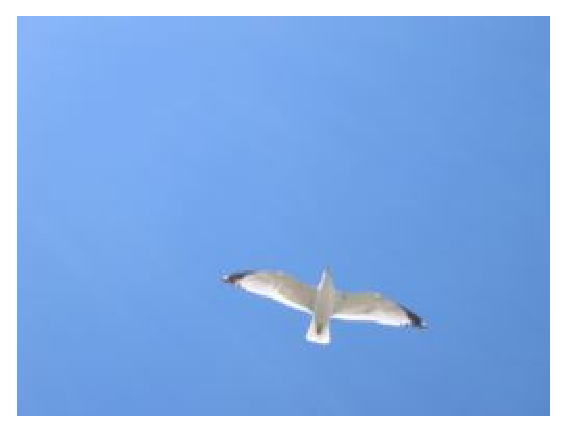
\includegraphics[width=5cm]{figs/seagull2.eps}
		         \caption{カモメ}
		         \label{fig:seagull}
	         \end{center}
         \end{wrapfigure}
	本研究の目的は、象の卵の殻について、生物、化学、物理、工学などの
	方面から多角的に調べることである。
	象の卵の殻は、80kgを超える体重の子象と、
	その栄養源である卵黄の大きな質量を支えるだけではなく、
	卵を暖める親の象の体重も支える必要がある。
	このため、象の卵の殻は、体重の軽い鳥類(図\ref{fig:seagull})の卵の殻とは本質的に異なる構造を持っていると
	考えられる。
	また、象の卵の殻の仕組みが解明されれば、
	\begin{itemize}
		\item 象の生態の解明、恐竜の卵の構造の理解(生物学)、
		\item 殻の化学生成反応の解明(化学)、
		\item 殻の原子レベルでの構造とC$_{60}$やナノクラスターとの関連の研究(物理)、
		\item 人工的に象の殻を作り、車の車体などに応用できる(工学)
	\end{itemize}
	など、科学、社会への影響は計り知れない。

	さて、象の卵の殻の強度については、すでに19世紀初めにロシアのキーファ・モキエーイチが
	考察していると、ゴーゴリが紹介している
	\cite{gogori}。
	しかし、この斬新で自由な発想にもとづく科学的考察に対し、
	トルストイは果敢にも、
	そういう考察がいかに論理的であろうとそれ自体間違っていて無駄である、
	と厳しく批判している
	\cite{torusutoi}。
	これは、既成概念にとらわれた、科学に対する挑戦ともとれるが、
	まだ進化論が現代の米国のように広く信じられていなかった
	帝政ロシアの時代にあっては、
	(進化論が米国で広く信じられているかどうかは、読み手の、文の解釈の仕方による)
	トルストイでさえも象の卵に対してこのような考えを
	持たざるを得なかったのは、理解できない事ではないと言わざるを得ないであろう。
	
	日本でも昔はナウマン象が生息しており、
	その名残は各地に残っている。
	例えば逢坂北部のある終点駅の駅前では、
	毎年年末になると図\ref{fig:egg_R}, \ref{fig:egg_L}に示すように
	象の卵の像のまわりを電飾するしきたりが残っている。
	(少し寄り目にし、右目で左の図、左目で右の図を見てください。
	なお、このように図や表を横に並べる方が、{\tt wrapfigure}を用いるより位置の調整が楽です。)
        \begin{figure}[h]
         	\begin{minipage}[t]{0.49\linewidth}
			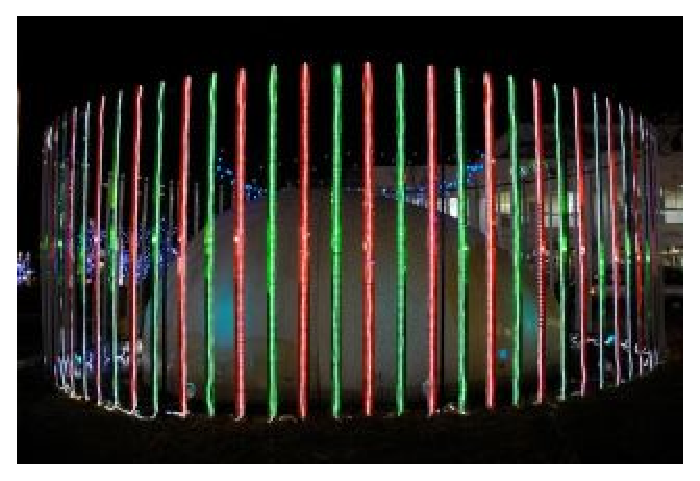
\includegraphics[width=\linewidth]{figs/egg_R.eps}
			\caption{右目用}
			\label{fig:egg_R}
		\end{minipage}
		\hspace{0.01\linewidth}
		\begin{minipage}[t]{0.49\linewidth}
			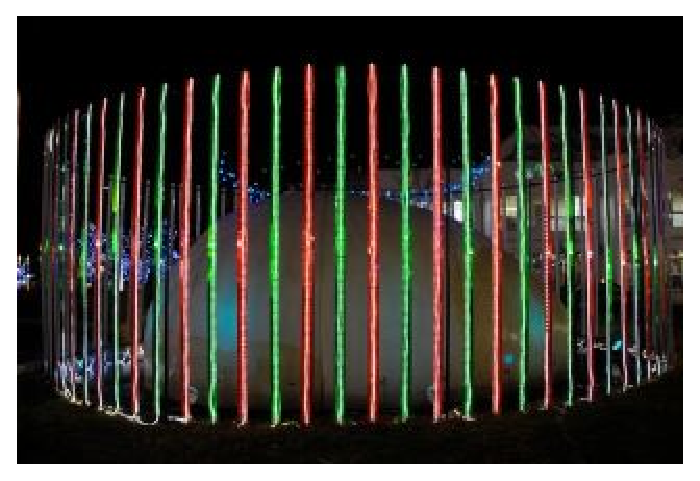
\includegraphics[width=\linewidth]{figs/egg_L.eps}
			\caption{左目用}
			\label{fig:egg_L}
		\end{minipage}
         \end{figure}

	また、寺村輝夫の研究\cite{teramura}によれば、昔、
	王子の誕生を祝って国民全員に卵焼きを提供すべく、
	軍隊を動員して象の卵を探させた王がいた。
	このときは孵化直後の子象は見つかったが、それが入っていた殻の発見には至っていない。
	人の家の裏庭の犬小屋を衛星写真で調べることさえもできなかった時代とあっては、
	この失敗も無理からぬことである。
	
	しかし今や、進化論は確立し、遺伝子の解析による派生の系統解析や
	犯人の特定ができる時代である。
	また、土を掘り返すことを基本としていた考古学でも、
	宇宙からナスカの近くに新たな地上絵を発見する時代である。
	このように、
	現代の科学技術を駆使すれば、マクロな広範囲に渡る精細な探索と、
	ミクロな遺伝子からの解析は可能であり、
	象の卵を世界に先駆けて発見することは、科学技術立国としての日本に課せられた使命でもある
	と言っても過言ではない。
	
	\vspace{1cm}
	\begin{thebibliography}{99}
		\bibitem{gogori} ゴーゴリ、「死せる魂」(1841).
		\bibitem{torusutoi} トルストイ、「人生論」(1886).
		\bibitem{teramura} 寺村輝夫、「ぼくは王様 - ぞうのたまごのたまごやき」.
	\end{thebibliography}
%end  研究目的 ====================
}

%====================================
%form: pdra_form_08.tex ; user: pdra_08_why_abroad.tex
%========== 海外特別研究員 =========
%===== p. 08 外国で研究する理由など =============
\section{外国で研究する理由など}
\section{外国で研究する事の意義}
\newcommand{\外国で研究する事の意義}{%
%begin  外国で研究する事の意義 (figureやtable使用可)===================
	私は今まで、象の卵の可能性について主に文献を漁って研究をしてきた。
	そうした長年の研究の末分かったことの一つは、日本に現在、自然界に生息
	する象はいないということである。
	最も最近生息した象はケナガマンモスのようであるが、
	祖父が子供の頃には既に絶滅していたそうである。
	マンモスの氷漬けの個体は北海道で見つかったが、卵は見つかっていない。
	また最近では2005年に愛知県のある会場で氷漬けの個体が見つかったが、
	これは実は密かにロシアから持ち込まれたものであり、国産象ではない。
	
	こうした経験から、象の卵を日本で探していても見つからないということを
	強く実感し、海外で研究する決心をした次第である。
	特に、象の卵を探す夢を子供の頃に私に与えてくれた
	Dr. Seussにぜひとも指導を仰ぎたく、師の元に行って研究を行う。
%end  外国で研究する事の意義 (figureやtable使用可) ====================
}

%form: pdra_form_09.tex ; user: pdra_09_need_rights.tex
%========== 海外特別研究員 =========
%===== p. 09 人権、法令など =============
\section{人権、法令など}
\subsection{人権の保護及び法令の遵守}
\newcommand{\人権の保護及び法令等の遵守への対応}{%
%begin  人権の保護及び法令等の遵守への対応 ===================
	象の卵のES細胞の培養、象のクローンの生成などは行わない。
	象個体を現地から持ち出すことはないので、ワシントン条約ならびに
        生物多様性条約に抵触しない。また、組換え実験は行なわないので、
        カルタヘナ議定書にも抵触しない。
%end  人権の保護及び法令等の遵守への対応 ====================
}

%form: pdra_form_10-11.tex ; user: pdra_10-11_publications.tex
%========== 海外特別研究員 =========
%===== p. 10-11 研究業績 =============
\section{研究業績}
%watermark: w14_pub_pdra
% 2008-03-08 Taku
% 2009-03-04 K.S.
% 2010-03-08 Taku: copied from PD
\renewcommand{\応募者の研究遂行能力}{%
%begin  研究遂行能力 ===================
	応募者は過去20年間、7つの海を隅から隅まで航海し、
	浅瀬から深海まで潜り、文字通り東西南北上下の3次元で
	シロナガスクジラの卵の探索を行ってきた。
	シロナガスクジラに飲み込まれそうになったり、海賊に捕まるなどの危険な目にも
	あったが、それにもめげず、研究を遂行してきた強靭な能力を有する。
%end  研究遂行能力 ====================
}

\subsection{学術雑誌(紀要・論文集等も含む)に発表した論文及び著書}
\newcommand{\学術雑誌等に発表した論文または著書}{%
%begin  学術雑誌等に発表した論文または著書===================
	
	\begin{enumerate}
		\item[](査読有り)%===========================
		\item \underline{H. Yukawa}$^1$, J. Kara$^2$,
				``Theory of Elephant Eggs'', 
				Phys.\ Rev.\ Lett. {\bf 800}, 800-804 (2005). 
				\label{pub:theoegg}
				
		\item F.~Ehrlich, \underline{H. Yukawa}$^1$,
				``You can't Lay an Egg If You're an Elephant'', 
				JofUR\\
				 ({\tt www.universalrejection.org}), {\bf N/A}, N/A (2002).

		\item[](査読なし)%=============================
		\item Kobo Abe$^3$, \underline{H. Yukawa}$^1$, 
				``仔象は死んだ'', 
				安部公房全集, {\bf 26}, 100-200, (2004).
	\end{enumerate}
	他5報
%end  学術雑誌等に発表した論文または著書 ====================
}

\subsection{学術雑誌等又は商業誌における解説・総説}
\newcommand{\学術雑誌等または商業誌における解説や総説}{%
%begin  学術雑誌等または商業誌における解説や総説===================
	\begin{enumerate}
		\item R.~Kipling, \underline{H. Yukawa},
				``The Elephant's Child (象の鼻はなぜ長い)'', 
				Nature, {\bf 999}, 777-779, (2003).
	\end{enumerate}
	他2件
%end  学術雑誌等または商業誌における解説や総説 ====================
}

\subsection{国際会議における発表}
\newcommand{\国際会議における発表}{%
%begin  国際会議における発表===================
	\begin{enumerate}
		\item $\circ$ 湯川秀樹、
			``Theory of Elephant Eggs'', 
			原始殻物理国際会議、
			カラチ、2006年2月

%		\item $\circ$ 湯川秀樹、Jacques-Yves Cousteau,
%			``How to search for whale eggs'',
%			国際海洋探索会議、ハワイ、2003年4月
	\end{enumerate}
	他1件
%end  国際会議における発表 ====================
}

\subsection{国内学会・シンポジウムにおける発表}
\newcommand{\国内学会やシンポジウムにおける発表}{%
%begin  国内学会やシンポジウムにおける発表===================
	\begin{enumerate}
		\item $\circ$ 湯川秀樹、朝永振一郎、
			「ほ乳類の真の意味」、
			ほ乳類学会、
			東京、2003年6月
	\end{enumerate}
	他3件
%end  国内学会やシンポジウムにおける発表 ====================
}

\subsection{特許}
\newcommand{\特許等}{%
%begin  特許等===================
	\begin{enumerate}
		\item[](公開中)
		\item 800800号、「クジラの卵を用いた深海潜水艇」\underline{湯川秀樹}、2003年4月
%		\item[] (申請中)
%		\item 8000000号、「象の卵を用いた(ひ・み・つ)」、\underline{湯川秀樹}、2007年4月
	\end{enumerate}		
%end  特許等 ====================
}

\subsection{その他の業績}
\newcommand{\その他の業績}{%
%begin  その他の業績===================
		\begin{enumerate}
			\item もうすぐもらえるで賞
		\end{enumerate}
%end  その他の業績 ====================
}

%===========================================================
% hook9 : right before \end{document} ============

%endUserFiles
% hook7 : right before including forms ============
 % for future maintenance

% pdra_forms
%=======================================
\ifthenelse{\boolean{BudgetSummary}\OR\boolean{klTypesetPage0}}{
	%============================================================
%  Warning cover page
%============================================================

\begin{picture}(0,0)(\KLOddPictureX,\KLPictureY)
	\KLParbox{100}{700}{550}{600}{t}{
		\LARGE
		提出前に次の行を以下のようにコメントアウトし、\\
		コンパイルし直してください。\\
		\hspace{2cm}\%\textbackslash setboolean\{BudgetSummary\}\{true\}\\
		\hspace{2cm}\%\textbackslash KLTypesetPage\{..\}\\
		\hspace{2cm}\%\textbackslash KLTypesetPagesInRange\{..\}\{..\}\\
	}
	\西暦
	\KLParbox{100}{550}{500}{500}{t}{
		\begin{center}
			\LARGE 予算と研究組織のまとめ \\
			\Large \today
		\end{center}
	}

	\KLTextBox{100}{500}{550}{300}{}{
		\Large
		研究種目: \研究種目\研究種別\研究種目後半\\
		研究期間: \研究開始年度(H\研究開始元号年度) 〜 H\研究期間の最終元号年度\\
		研究課題名:「\研究課題名」\\
		研究代表者:\研究代表者氏名\\
		研究機関名:\研究機関名\\
	}
\end{picture}
\clearpage


}{}

\KLInputIfPageInRangeIsSelected{1}{2}{forms/pdra_form_04-05}
\KLInputIfPageInRangeIsSelected{3}{4}{forms/pdra_form_06-07}
\KLInputIfSelected{5}{forms/pdra_form_08}
\KLInputIfSelected{6}{forms/pdra_form_09}
\KLInputIfPageInRangeIsSelected{7}{8}{forms/pdra_form_10-11}
	
%========================================


%endFormatFile

% hook9 : right before \end{document} ============
 % for future maintenance
\end{document}
